\documentclass{article}
\usepackage{enumerate}
\title{Project Report: Audio Extraction and Shuffling}
\author{Sudarshan Shivashankar}
\date{\today}
%\documentclass{article}
\usepackage{graphicx}

\begin{document}
\maketitle

\section{Introduction}
The purpose of this project is to extract audio from a series of video files and play them in a shuffled order. The project utilizes the MoviePy library to extract audio from video files and the NumPy library to shuffle the order of the audio files. The extracted audio files are saved in WAV format and played using the 'aplay' command line utility.

\section{Objectives}
The main objectives of this project are as follows:
\begin{enumerate}
  \item Extract audio from a series of video files using the MoviePy library.
  \item Utilize the NumPy library to shuffle the order of the audio files.
  \item Save the extracted audio files in WAV format for playback.
  \item Implement a loop that plays the shuffled audio files until the user chooses to stop.
  \item Provide documentation and clear instructions for the user to understand and use the program effectively.
\end{enumerate}

\section{Methodology}
The project was implemented using the following steps:

\subsection{Audio Extraction}
The program uses the MoviePy library to extract audio from a series of video files. The \texttt{extract\_audio} function takes the path of the video file and the desired output file path as input. It extracts the audio from the video and saves it as a WAV file.

\subsection{Array Shuffling}
A list of numbers from 0 to 19 is created. This list is converted to a NumPy array using \text{np.array()}. The \text{np.random.shuffle()} function shuffles the array in-place, changing the order of the numbers randomly.

\subsection{Audio Playback}
The shuffled array is converted back to a list using \text{.tolist()}. The program then loops through the shuffled numbers and performs the following steps for each number:
\begin{enumerate}
  \item Prints the current number.
  \item Constructs the file paths for the input video file (\text{mp4\_file\_path}) and the output audio file (\text{output\_file\_path}).
  \item Calls the \text{extract\_audio} function to extract the audio from the video and save it as a WAV file.
  \item Uses the \text{subprocess.call()} function to play the extracted audio file using the 'aplay' command line utility.
  \item Prompts the user to enter 'q' if they want to stop playing the songs. If 'q' is entered, the loop breaks; otherwise, it continues.
\end{enumerate}

\section{Results}
The program successfully extracts audio from a series of video files and shuffles the order of the audio files. The shuffled audio files are played one by one using the 'aplay' command line utility. The user can choose to stop playing the songs by entering 'q' when prompted.



\begin{figure}[h]
  \centering
  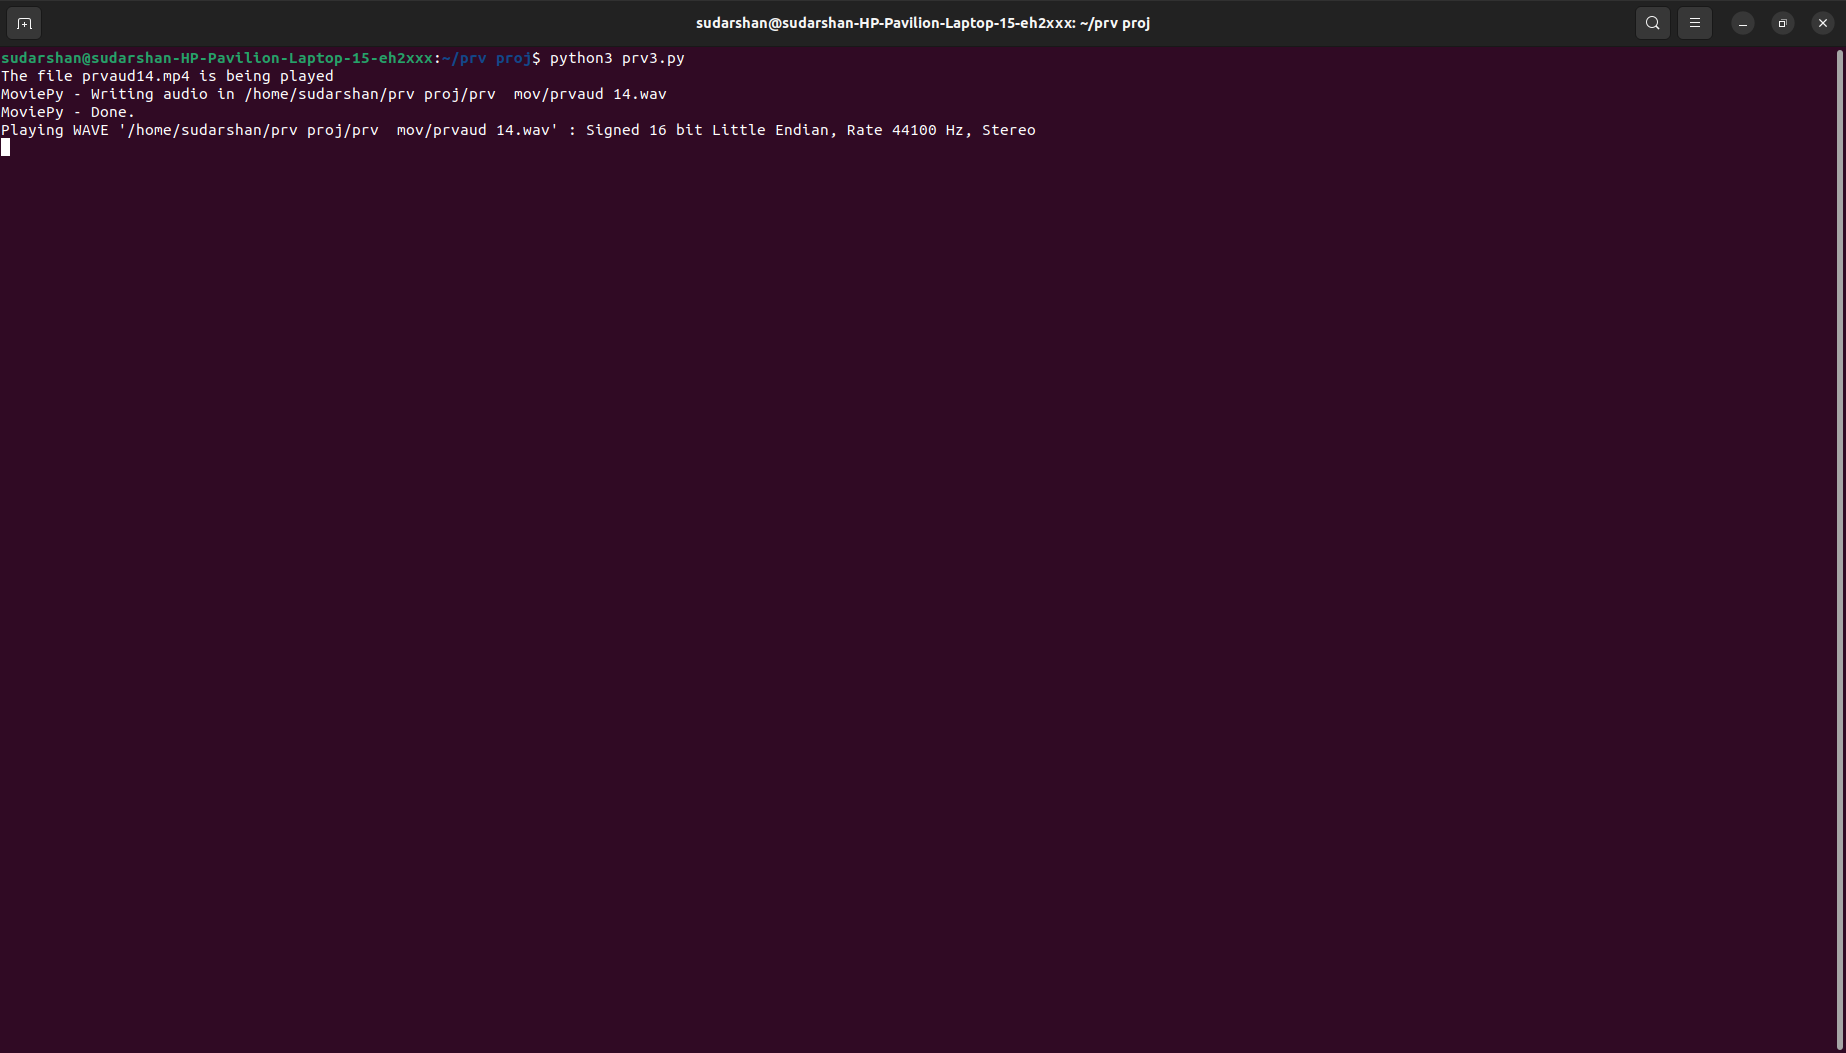
\includegraphics[width=0.5\textwidth]{/home/sudarshan/prv proj/projsoft/img/prvimg1.png}
  \caption{Playing a random song.}
  \label{fig:sample}
\end{figure}


\begin{figure}[h]
  \centering
  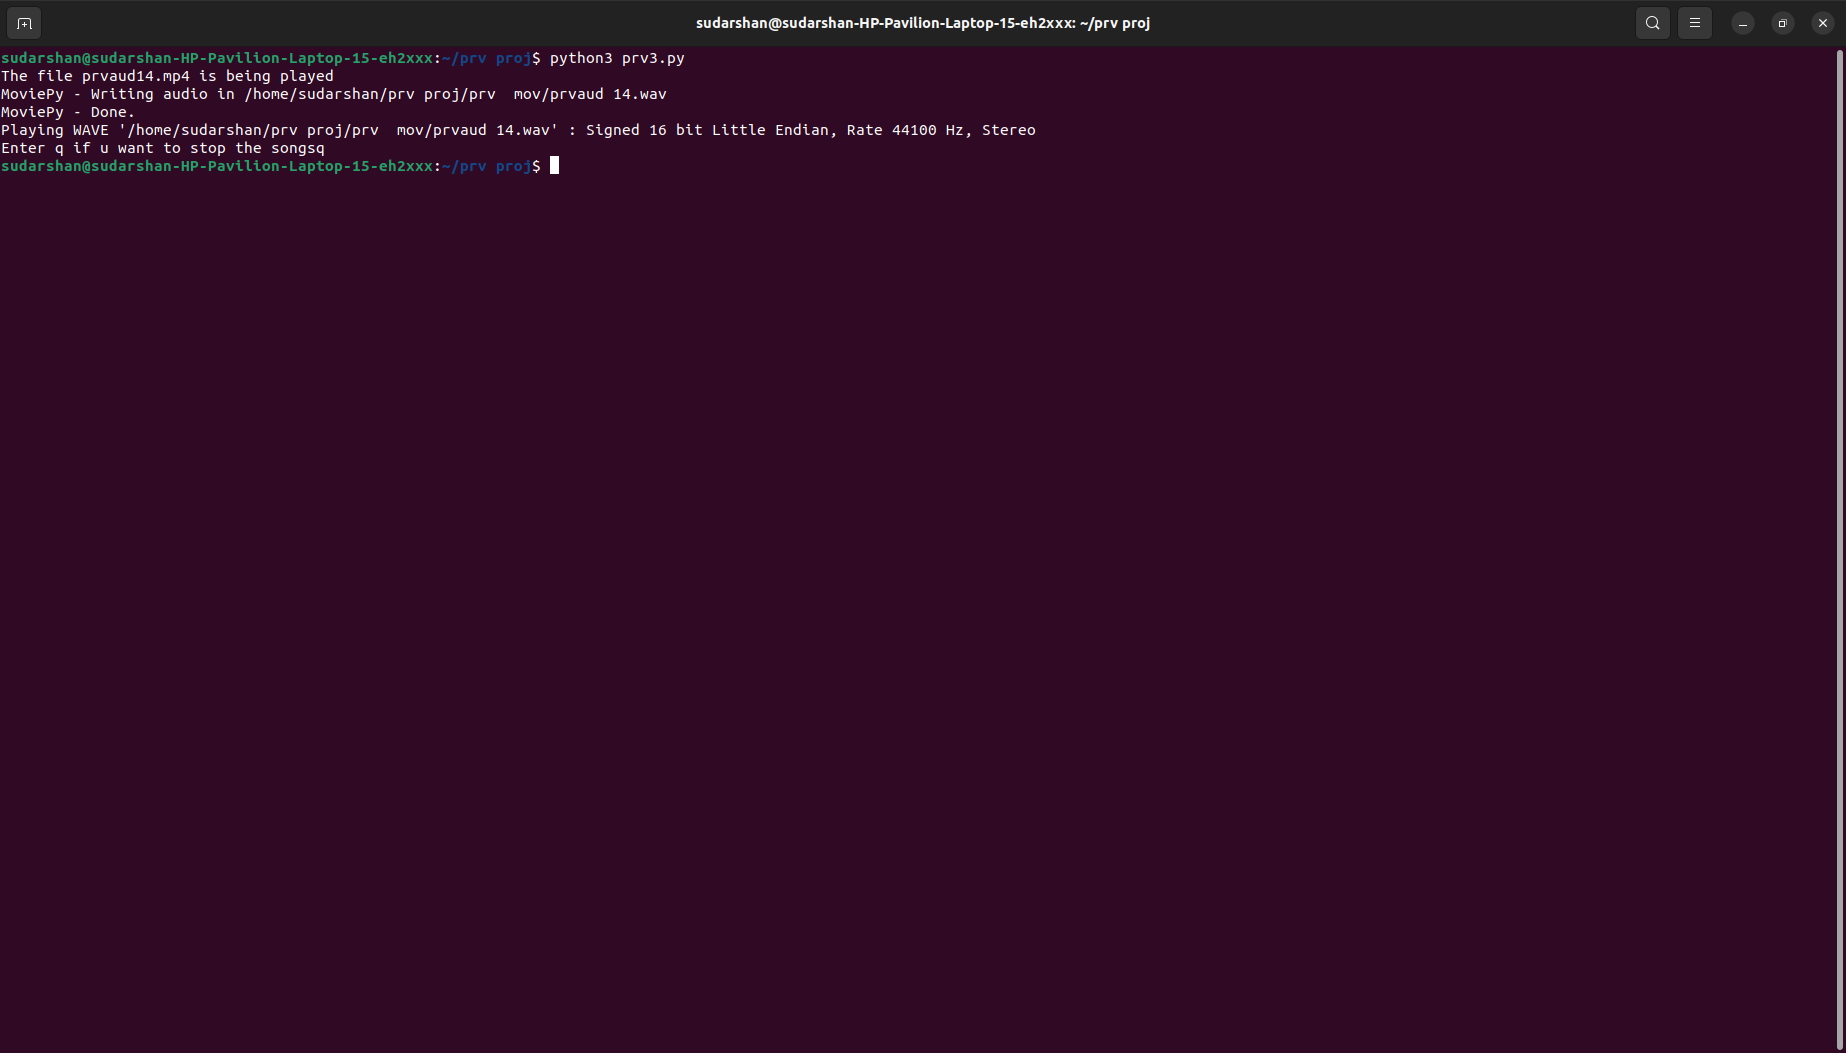
\includegraphics[width=0.5\textwidth]{/home/sudarshan/prv proj/projsoft/img/prvimg2.png}
  \caption{ Displaying option to quit the playlist}
  \label{fig:sample}
\end{figure}

\section{Conclusion}
The project accomplished the goal of extracting audio from video files, shuffling the order of the audio files, and playing them using the 'aplay' utility. The program provides a simple and interactive way to enjoy shuffled audio playback. Users can modify the program to work with their own collection of video files and enjoy a randomized audio experience.

\section{Future Enhancements}
\begin{enumerate}
  \item Implement a graphical user interface (GUI) for a more user-friendly experience.
  \item Add support for additional audio formats and playback options.
  \item Integrate with online music platforms for automatic extraction and shuffling of audio files.
  \item Provide options for customizing the shuffling algorithm and playback settings.
\end{enumerate}

\section{References}
\begin{enumerate}
  \item MoviePy documentation: \text{https://zulko.github.io/moviepy/}
  \item NumPy documentation: \text{https://numpy.org/doc/}
  \item subprocess module documentation: \text{https://docs.python.org/3/library/subprocess.html}
\end{enumerate}

\end{document}
